\chapter{Исследовательский раздел}
\label{cha:research}

\section{Тестирование производительности}

\section{Описание используемых шаблонов проектирования}

\subsection{Шаблон <<вызов переопределенного метода>>}

Представляет ситуацию, когда вызывается метод интерфейса,
для которого имеется реализация в производном классе.
Граф шаблона представлен на рисунке~\ref{fig:OverriddenMethodCall-graph}.

\begin{figure}[!ht]
\centering
\includegraphics[width=0.6\textwidth]{inc/OverriddenMethodCall-graph.pdf}
\caption{Граф шаблона <<вызов переопределенного метода>>}
\label{fig:OverriddenMethodCall-graph}
\end{figure}

\subsection{Шаблон <<абстрактная фабрика>>}

Предоставляет интерфейс для создания групп связанных или зависимых объектов,
не указывая их конкретный класс.
Граф шаблона представлен на рисунке~\ref{fig:AbstractFactory-graph}.

\begin{figure}[!ht]
\centering
\includegraphics[width=0.6\textwidth]{inc/AbstractFactory-graph.pdf}
\caption{Граф шаблона <<абстрактная фабрика>>}
\label{fig:AbstractFactory-graph}
\end{figure}

\subsection{Шаблон <<адаптер>>}

Конвертирует интерфейс класса в другой интерфейс, ожидаемый клиентом.
Позволяет классам с разными интерфейсами работать вместе.
Граф шаблона представлен на рисунке~\ref{fig:Adapter-graph}.

\begin{figure}[!ht]
\centering
\includegraphics[width=0.6\textwidth]{inc/Adapter-graph.pdf}
\caption{Граф шаблона <<абстрактная фабрика>>}
\label{fig:Adapter-graph}
\end{figure}

\subsection{Шаблон <<мост>>}

Разделяет абстракцию и реализацию так, чтобы они могли изменяться независимо.
Граф шаблона представлен на рисунке~\ref{fig:Bridge-graph}.

\begin{figure}[!ht]
\centering
\includegraphics[width=0.6\textwidth]{inc/Bridge-graph.pdf}
\caption{Граф шаблона <<мост>>}
\label{fig:Bridge-graph}
\end{figure}

\subsection{Шаблон <<посетитель>>}

Представляет операцию, которая будет выполнена над объектами группы классов.
Даёт возможность определить новую операцию без изменения кода классов,
над которыми эта операция производится.
Граф шаблона представлен на рисунке~\ref{fig:Visitor-graph}.

\begin{figure}[!ht]
\centering
\includegraphics[width=\textwidth]{inc/Visitor-graph.pdf}
\caption{Граф шаблона <<посетитель>>}
\label{fig:Visitor-graph}
\end{figure}

\section{Поиск шаблонов проектирования в существующих программах}

\subsection{Проект <<java-design-patterns>>}

Проект находится в открытом доступе, размещен на ресурсе
github.com~\cite{java-design-patterns}.
Интересен тем, что содержит сборник из 48 примеров реализации различных
шаблонов проектирования на языке \textbf{Java},
что очень хорошо подходит для проверки работы программного комплекса.
Здесь можно увидеть некоторые из особенностей реализации шабонов,
поэксперементировать с разными представлениями шаблона.

\subsubsection*{Поиск шаблона <<вызов переопределенного метода>>}

\subsubsection*{Поиск шаблона <<абстрактная фабрика>>}

Первый реализованный пример шаблона в проекте.
Реализация совпадает с разными описаниями.
Шаблон находится, результат представлен на рисунке~\ref{fig:java-design-patterns-abstract-factory}.

\begin{figure}[!ht]
\centering
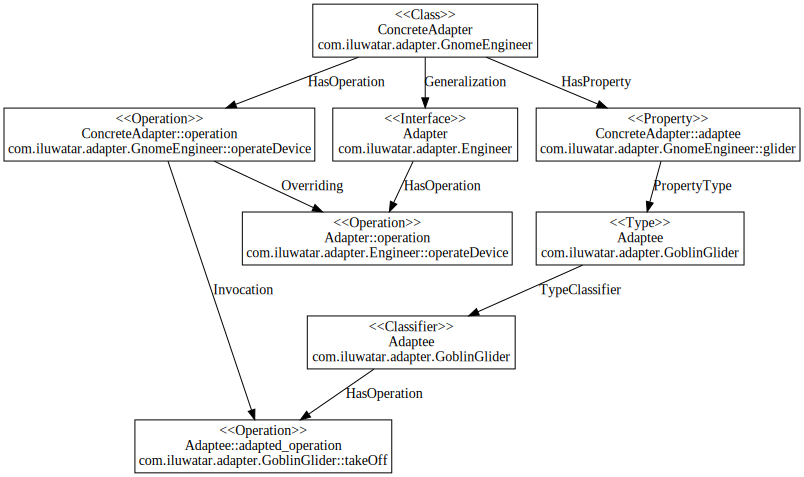
\includegraphics[width=\textwidth]{inc/java-design-patterns-adapter.pdf}
\caption{Результат поиска шаблона проектирования <<абстрактная фабрика>> в примере его реализации}
\label{fig:java-design-patterns-abstract-factory}
\end{figure}

\subsubsection*{Поиск шаблона <<адаптер>>}

Для шаблона есть пример, и шаблон в нем находится.
Результат представлен на рисунке~\ref{fig:java-design-patterns-adapter}

\begin{figure}[!ht]
\centering
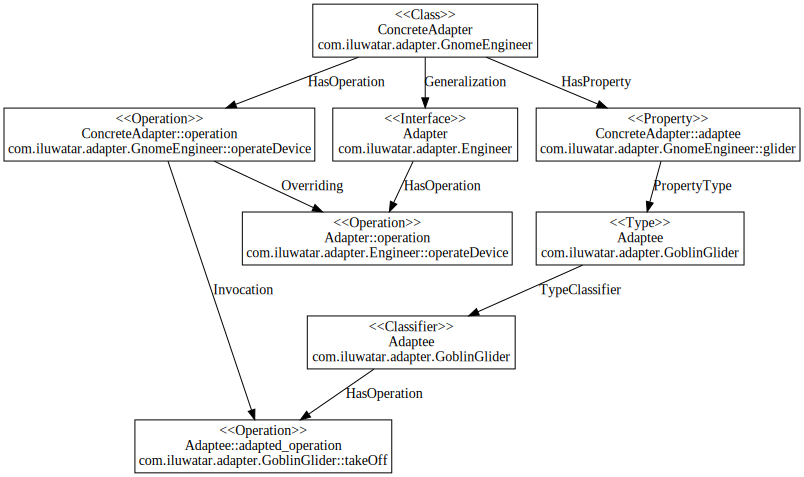
\includegraphics[width=\textwidth]{inc/java-design-patterns-adapter.pdf}
\caption{Результат поиска шаблона проектирования <<адаптер>> в примере его реализации}
\label{fig:java-design-patterns-adapter}
\end{figure}

\subsubsection*{Поиск шаблона <<мост>>}

В примере реализации не найден, но найден в других примерах.
Проблема заключается в том, что используется дополнительное обобщение,
чтобы не было дублирования кода.
Класс \textbf{Abstraction} разделен на две части: базовый абстрактный класс
\textbf{MagicWeapon},
который совязан ассоциацией с \textbf{MagicWeaponImp},
являющимся интерфейсом \textbf{Implementor};
и конкретными реализацими: \textbf{BlindingMagicWeapon},
\textbf{FlyingMagicWeapon}, \textbf{SoulEatingMagicWeapon}.
Здесь требуется механизм, который позволит описать класс так,
все ассоциации базового класса также являются и ассоциациями производного.
Нужна сущность, которая может объединять иерархии наследования классов в
некоторый надкласс.
UML-диаграммы классов не предоставляют такого механизма.
В данной работе эта проблема осталась не решенной.

Шаблон был найден в следующих примерах:
\begin{itemize}
\item adapter;
\item decorator;
\item intercepting-filter;
\item mediator;
\item model-view-presenter;
\item null-object;
\item poison-pill;
\item property;
\item service-layer;
\item state;
\item strategy.
\end{itemize}

\subsubsection*{Поиск шаблона <<посетитель>>}

Шаблон реализован в специальном примере и находится.
Результат представлен на рисунке~\ref{fig:java-design-patterns-visitor}

\begin{figure}[!ht]
\centering
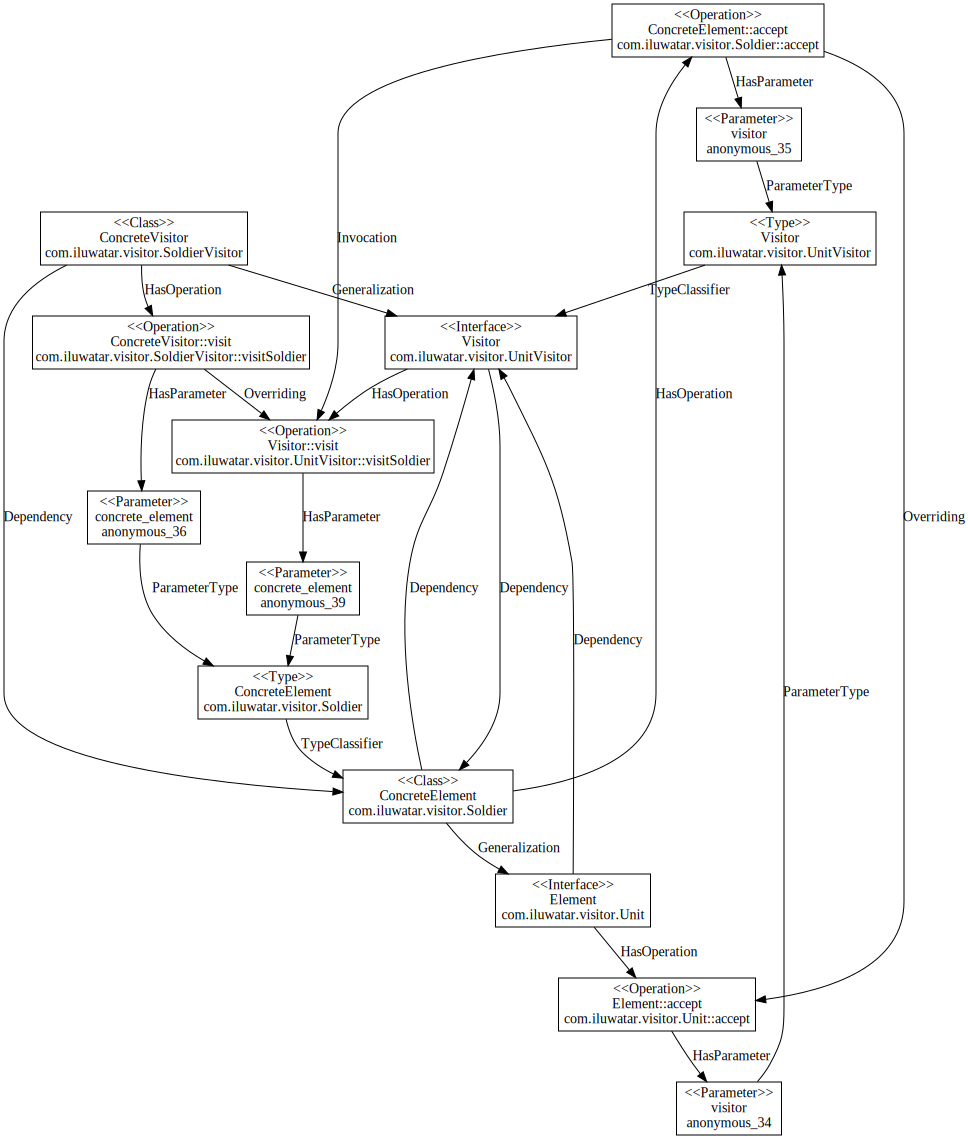
\includegraphics[width=\textwidth]{inc/java-design-patterns-visitor.pdf}
\caption{Результат поиска шаблона проектирования <<посетитель>> в примере его реализации}
\label{fig:java-design-patterns-visitor}
\end{figure}

\subsection{Библиотека <<Apache BCEL>>}

Исследовалась в качестве примера реального проекта.
Модель проекта в \textbf{YAML}-формате занимает 4,1 МБ.
Граф модели состоит из 7700 вершин и 52000 дуг.
